\documentclass[fleqn,twoside,reqno]{article}
\usepackage[margin=1in]{geometry}  % Set margin to 1 inch on all sides
\usepackage{setspace}
\usepackage{amsmath, amssymb}
\usepackage{graphicx}
\usepackage{geometry}
\usepackage{afterpage}
\usepackage{xcolor}
\usepackage{multirow}
\usepackage{tabularx}
\usepackage{booktabs, array, rotating}
\usepackage{makecell}
\usepackage{adjustbox}
\usepackage[para]{threeparttable}
\usepackage[colorlinks=true, linkcolor=blue, citecolor=blue, urlcolor=blue]{hyperref}
\usepackage{cleveref}
%Create running head
\usepackage{fancyhdr}
\pagestyle{fancy}
\fancyhf{}% Clear header/footer
\fancyhead[R,L]{%
  \ifodd\value{page}\relax
    ADOPTION \& INTENSITY OF AGRO-ECOLOGICAL PEST MANAGEMENT% Odd page header
  \else
    OWILI \textit{ET AL}. (2024)% Even page header
  \fi}
  \fancyhead[RE,LO]{\textbf{\thepage}} % Page number on the top outer corner
\renewcommand{\headrulewidth}{0pt}

\usepackage{silence}
\WarningsOff[everypage]% Suppress warnings related to package everypage
%Removing unnecessary whitespaces
\raggedbottom
% Change font
\usepackage{epigrafica}
\usepackage[LGR, OT1]{fontenc}
%Insert a preprint watermark
%\usepackage{background} % For watermarks
% Define the watermark content and position
%\backgroundsetup{
% scale=5, color=black, opacity=0.1, angle=45, position=current page.center,
% contents={\textbf{Preprint not peer reviewed}}, % Watermark content
%}
%ORCiD
\newcommand{\orcid}{
\includegraphics[width=8pt]{ORCID}} % ORCID ID
% Redefine the abstract environment
\renewenvironment{abstract}
 {\begin{center}\large\MakeUppercase{\abstractname}\end{center}
  \list{}{\leftmargin=1.5em\rightmargin=1.5em \parsep=0pt \relax}
  \item\relax}
 {\endlist}
%Hanging keywords
\usepackage{parskip}
\newenvironment{Keywords}{%
\sbox0{\textbf{Keywords}: }%
\list{}{\labelwidth\wd0 \leftmargin\wd0 \labelsep 0pt }
             \item[\usebox0]}
               {\endlist}
%References
\usepackage[backend=bibtex, maxcitenames=2, style=ieee, citestyle=authoryear, uniquename=init]{biblatex}
\addbibresource{references.bib}
%\usepackage{lineno}
%\usepackage{etoolbox} % For patching \linenumberfont
%\renewcommand\linenumberfont{\normalfont\footnotesize}
% If you're using an older version of lineno, you might need to use \patchcmd instead
% \patchcmd{\linenumberfont}{\normalfont}{\normalfont\footnotesize}{}{}
% Customize line numbering format to right-align line numbers
%\renewcommand\linenumberfont{\normalfont\footnotesize\sffamily\color{blue}}
%\rightlinenumbers % Right line numbering
%\linenumbers % Turn on line numbering
\title{\fontsize{14}{14}\selectfont \textbf{Factors influencing adoption of agro-ecological pest management options for mango fruit fly under information constraints: A two-part fractional regression approach}}
\author{
\begin{tabular}{p{\dimexpr\textwidth-2\tabcolsep}}
Sulman Olieko Owili\textsuperscript{a,b}\thanks{Corresponding author. Email: \texttt{oliekosulman@gmail.com}} \href{https://orcid.org/0000-0001-7401-5326}\orcid{}, 
David Jakinda Otieno\textsuperscript{a}\href{https://orcid.org/0000-0001-9904-0819}\orcid{}, 
Evans Ligare Chimoita\textsuperscript{a}, 
Frederick Philbert Baijukya\textsuperscript{b} \\
\medskip
\textsuperscript{a}Department of Agricultural Economics, University of Nairobi, P.O Box 29053--00625, Kangemi, Kenya; \\
\textsuperscript{b}International Institute of Tropical Agriculture, P.O Box 30709--00100, Nairobi, Kenya
\end{tabular}
}

\date{\today}
\begin{document}
\maketitle
\begin{abstract}
The catalytic effect of climate change on the emergence and prevalence of invasive alien pests, coupled with weak pesticide regulatory frameworks in developing countries, has necessitated a transition towards sustainable pest management. Agro-ecological pest management (APM) is a nature-based, cost-effective alternative for systemic pest challenges, such as mango fruit fly invasion. We applied a two-part fractional regression to sequentially model APM adoption and intensity decisions on a sample of 423 smallholder mango orchard managers from Makueni County, Kenya. Despite the potential of APM, the results suggest that only 56.7\% of the farmers adopted it. The average adopter applied 25\% of the APM practices concurrently. Farmers’ socio-psychological attributes significantly influenced both adoption and intensity decisions. Perceptions of technology attributes, training and group membership dominated the adoption decision, while attitudes toward orchard biodiversity, prospects, and information constraints were the main drivers of the intensity of uptake. To support transition from use of synthetic insecticides to APM measures, policymakers should create more opportunities for training and knowledge co-creation, especially through social networks and gender-disaggregated participatory group approaches.\\
\end{abstract}

\begin{Keywords} Agro-ecological pest management, behavioural change, fruit fly, intensity of adoption, mango, two-part fractional regression
\end{Keywords}

\textbf{JEL Classification}: C34, Q12, Q15, Q16, Q54, Q57

\doublespacing  % Set double spacing
\section{Introduction}\label{sec:1}
\fontsize{12}{14}\selectfont % Set body text font size to 12pt with 14pt line spacing
Invasive alien pests pose an increasing threat to human livelihoods, particularly as climate change-induced ecosystem disturbances and transboundary trade pathways expand and intensify (\cite{Early2016, Skendzic2021}). Historically, pest invasions have been known for their association with high economic consequences resulting from yield loss and abatement costs. For instance, between 1970 and 2017, an annual average of USD 18.6 billion was estimated to be lost directly to damage caused by invasive species, including pests, while an additional USD 1.4 billion was estimated to be incurred in management costs globally (\cite{Diagne2021}). The economic impacts associated with invasive pests are particularly concerning for sub-Saharan Africa (SSA) economies, where the agricultural sector contributes 20--50\% of the gross domestic product (GDP) (\cite{Giller2020}) and employs approximately 53\% of the workforce (\cite{Srinivasan2022}). These effects are further compounded by the existence of weak regulatory frameworks and inadequate response mechanisms for the containment and eradication of invasive pests (\cite{Ndlela2022}).

The conventional management of systemic pest challenges has predominantly relied on the application of synthetic pesticides (\cite{Schreinemachers2017}). However, over time, the widespread and intensive use of synthetic pesticides has negatively affected agroecosystems by exacerbating climate change and biodiversity loss (\cite{Heimpel2013, Skendzic2021}). Extensive pesticide use has also contributed to the ‘pesticide treadmill\footnote{This is a situation in which extensive use of pesticides results in pest resistance, compelling farmers to apply larger quantities and often more toxic pesticides to control pest populations.}’, which has diminished natural pest control efforts (\cite{Bakker2020}). Projections indicate that by 2030, the hidden costs associated with conventional food systems could reach up to USD 13 trillion per year (\cite{Rockstrom2020}).

Agro-ecological pest management (APM) represents a paradigm shift from conventional pest management. Broadly, APM is a systemic approach that prioritises prophylactic control options for long-term pest management through the utilisation of contextualised bio-rational strategies that are compatible with existing methods and adaptable to future food production bottlenecks (\cite{Belmain2022}). By design, APM practices are hybridised on both indigenous and scientific knowledge (\cite{Deguine2021, Wezel2009}), with emphasis on the utilisation and recycling of on-farm and locally available inputs to reduce reliance on chemical pesticides. Thus, this approach is viable, particularly for smallholder farmers in resource-limited settings.

In SSA, mango (\textit{Mangifera indica L.}) is cultivated predominantly by smallholders under rain-fed conditions, constituting up to 90\% of the total annual production (\cite{Ndlela2022}). The crop ranks second among fruit crops in Kenya, following bananas in both value and volume. In 2020, its annual production value was USD 154 million --representing 17.34\% of the total fruit value and 8.64\% of the horticultural GDP in the country (\cite{HCD2021}).

The major impediment to mango productivity and marketing is the oriental fruit fly \textit{Bactrocera dorsalis} (Diptera: Tephritidae). This pest is highly invasive, and its fecund and polyphagous traits endow it with comparative advantages over its intraspecific competitors (\cite{Mutamiswa2021}). This pest has been reported to reduce yields by between 30 and 90\% (\cite{Vayssieres2009}). In the African continent alone, approximately USD 2 billion is estimated to be lost annually due to quarantine and self-bans associated with the pest (\cite{Korir2015}). Consequently, there is an urgent need to mitigate the impacts of \textit{B. dorsalis} and enhance the sustainability of the mango value chain.

At the farm level, the decision to transition to sustainable technologies, such as APM, is primarily driven by the economic advantages offered by alternative technologies. However, it is widely recognised that the main relative advantage of environmentally sustainable practices is the delivery of public goods in the form of positive externalities such as ecosystem services. Therefore, decisions to adopt eco-friendly alternatives often have economic consequences and are generally more controlled (\cite{Dessart2019}). Voluntary adoption under such circumstances are likely to be under the influence of farmer’s intrinsic motivations (\cite{Ejelov2022, Meijer2015, Runhaar2017, Schoonhoven2018}).

Our contribution to the literature is twofold. First, the extant literature on the voluntary uptake of environmentally sustainable pest management technologies by smallholder farmers that accounts for the behavioural attributes of decision makers has predominantly focused on the intention to adopt (\cite{Despotovic2019, Khan2021, Punzano2021}) and willingness to pay for (\cite{Muriithi2021, Nyangau2022, Petrescu2019}) pest management technologies. Although self-reported intentions and willingness to adopt a technology can predict observed behavioural patterns, farmers may overstate their intentions and willingness in an attempt to report ‘socially acceptable’ behaviours (\cite{Khan2021,Petrescu2019}). Largely, studies on actual adoption decisions have overlooked the critical role of the intrinsic motivations of decision makers. Our analysis accounts for a number of latent covariates that encompass this aspect.

Second, as a departure from the literature, which often models pest management decisions as single-stage processes, we introduce pest management decisions into a sequential decision framework, allowing each decision stage to be influenced by separate data-generating processes (DGPs). Within this framework, we adopt a more nuanced approach by focusing on the orchard manager as the unit of analysis, following \cite{Miriti2021}. An orchard manager is defined as the individual responsible for the majority of decisions related to orchard-level activities. This approach relaxes the often-restrictive assumption that the household head is the primary decision maker in agricultural enterprises.

The primary objective of this study was to analyse the determinants of the adoption and intensity of APM practices for mango fruit fly suppression among smallholder farmers under information constraints. Specifically, we tested the hypotheses that: (i) socio-psychological factors have no influence on APM adoption and intensity decisions, and (ii) information constraints do not influence the level of uptake of APM technology.

The remainder of the paper is organised as follows: In section \ref{sec:2}, we discuss the research methodology, including a brief description of the study area, the sampling procedure and data collection, the variables employed in the study and the analytical framework. We then present and discuss our results in section \ref{sec:3}, before concluding in section \ref{sec:4} with a brief discussion of the implications of our findings for practice, policy and future research.

\section{Data and methods}\label{sec:2}
\subsection{Study area}
This study was conducted in Makueni County, located in the southeastern region of Kenya (Figure \ref{fig:1}). The county covers a total area of $8,176.7\mathrm{km^2}$, 62\% of which is classified as arable land. The upper part of the county features fertile soil and experiences an average annual rainfall ranging from 800 to 1200 mm, with annual temperatures ranging from 17 to $30^\circ$C (\cite{County2022}). These conditions not only favour the cultivation of horticultural crops such as mango but also contribute to high pest incidences. Makueni County is home to approximately $28,696$ smallholder households practising rain-fed farming, and is the leading producer of mango in Kenya, contributing up to 19.7\% of the annual production in 2020 (\cite{HCD2021}).
\begin{figure}[!ht]
  \centering
  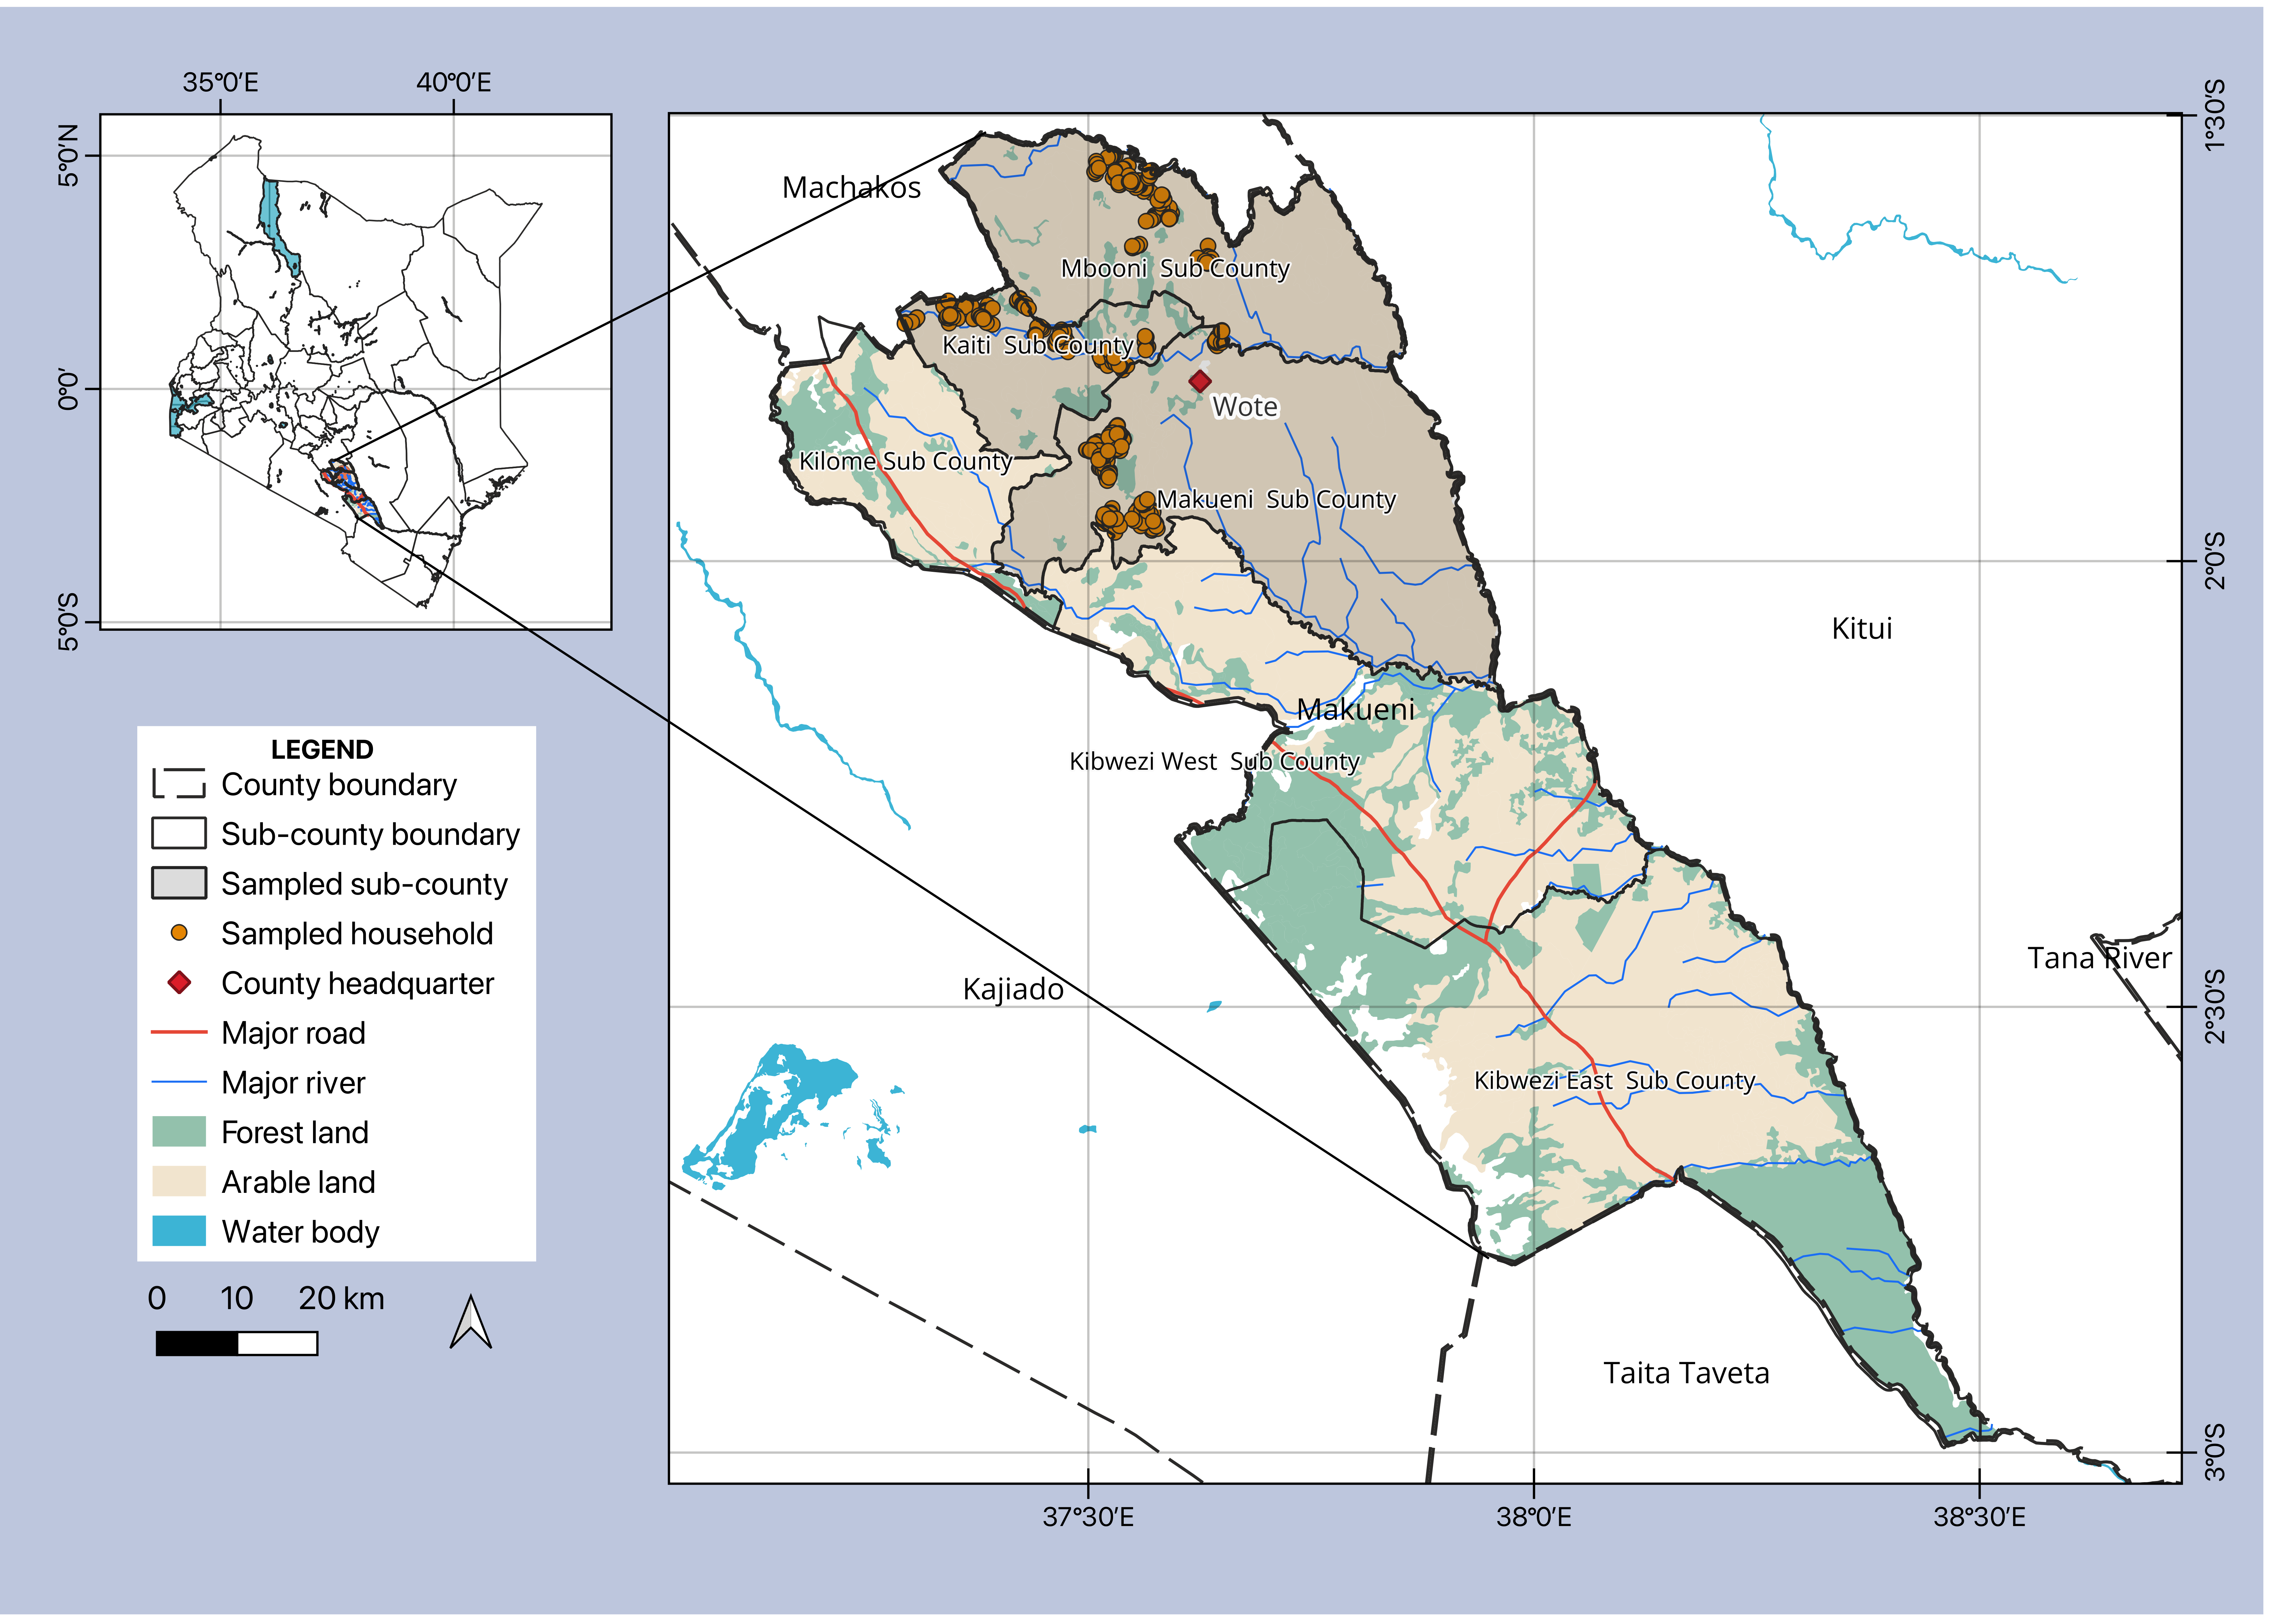
\includegraphics[width=1\textwidth]{Fig.1.png}
  \caption{Map of the study sites in Makueni County, Kenya}
  \label{fig:1}
\end{figure}

\subsection{Sampling technique and data collection}
We employed a cross-sectional survey design with a multistage sampling procedure. In the first two stages, purposive sampling was used to select Makueni County and the sub-counties of Makueni, Mbooni, and Kaiti. In the third and fourth stages, simple random sampling procedures were employed to select six wards and twelve sub-wards, respectively, from the three sub-counties. A systematic random sampling approach was implemented at the final stage, during which every third orchard manager was selected from each sub-ward.

The study utilised the \cite{Yamane1967} formula to determine the required sample size $n$ as:
\begin{align}
n &= \frac{N}{1 + N \cdot e^2}
\end{align}
At the 95\% confidence level, the minimum sample size required was 395. However, we adjusted this value by a factor of 1.10 to 434 orchard managers to address potential issues related to incomplete questionnaires, nonresponses and outliers. This adjustment coefficient has been utilised in previous literature (see \cite{Ojwang2021}). The data were collected between August and September 2023 and involved face-to-face interviews by trained enumerators using a pretested questionnaire. Informed consent was obtained from the respondents prior to the interviews. The questionnaire captured information such as the household and respondent demographics, asset endowment, access to institutional services, awareness, perceptions, attitudes and knowledge, adoption of agro-ecological practices, input use and mango production. All the surveyed orchard managers had observed fruit fly damage in their orchards at least 5 years before the survey.

\subsection{Theoretical framework}
The study was anchored on the von Neumann-Morgenstern expected utility theory, which posits that a decision-making unit (DMU) evaluates the expected utility of potential outcomes to maximise profit when choosing between risky and uncertain prospects (\cite{Neumann1944}). Risks in pest management are associated with yield loss and management costs due to pest damage, as well as health and market uncertainties. Due to loss aversion, the uncertainty associated with innovations such as APM makes them less appealing to smallholder farmers than conventional alternatives (\cite{Alwang2019}). Shifting to APM can be risky, particularly when there are limited or no insurance safety nets in place, as is the case in SSA. Consequently, decisions to adopt such innovations are primarily based on expectations (\cite{Feder1979}). Choices under such scenarios involve varying degrees of risk and are often linked to multifaceted outcomes. Therefore, prior to adoption and intensity decisions, rational farmers are assumed to evaluate options based on the available information to understand the probability distribution of their outcomes.

Suppose we denote the consequences of adopting a fruit fly management technology by a finite set $C = \{c_{i1}, c_{i2}, \ldots, c_I\}$, and let the set of all available alternatives be represented by $A = \{a_{\text{APM}}, a_{\text{Conventional}}, \ldots, a_I\}$. Then, adoption is associated with a probability distribution over consequences such that:
\begin{align}
\begin{split}
a: C & \longrightarrow [0, 1] \quad \text{with} \quad \sum_{c \in C} a^*(c)\\
\sum_{c \in C} p_i &= \sum_{c \in C} q_i = \ldots = 1 \quad \forall p_i \geq 0, q_i \geq 0
\end{split}
\label{eq:2}
\end{align}
where $p_i$ and $q_i$ represent the probabilities of obtaining result $c_i$ when APM or alternative methods are adopted, respectively. The von Neumann-Morgenstern utility function $u(\cdot)$ is defined as $u: C \longrightarrow \mathbb{R}$ such that:
\begin{align}
\begin{split}
\mathbb{E}[U(a)] &= \sum_{c \in C} a(c) u(c) \quad \forall a_{APM}, a_{\text{Conventional}}, \ldots \in A\\
\mathbb{E}[U(a_{\text{APM}})] &= \sum_{c \in C} p_i u(c_i) \quad \text{and} \quad
\mathbb{E}[U(a_{\text{Conventional}})] = \sum_{c \in C} q_i u(c_i)
\end{split}
\label{eq:3}
\end{align}
The expected utility function $\mathbb{E}[U(\cdot)]$ takes the form $\mathbb{E}[U]: a \longrightarrow \mathbb{R}$, and $A$ is a closed, bounded, and compact subset of $\mathbb{R}^n$, where $n = |C|$. The primary objective of a risk-averse DMU is to maximise the expected utility by adopting a technology from the set A of alternatives if its expected utility is higher than that of other alternatives:
\begin{align}
a_{APM} \succ a_{\text{Conventional}} \Leftrightarrow \mathbb{E}[U(a_{\text{APM}})] - \mathbb{E}[U(a_{\text{Conventional}})] > 0 
\end{align}
Since the adoption decision is dichotomous, modelling is typically performed using discrete choice models such as a probit or logit.

\subsection{Empirical framework}
\subsubsection{\textit{Sequential decision process}}
We considered the adoption and intensity of APM decisions as separate and sequentially made by orchard managers, assuming dissimilar DGPs. Adoption was voluntary, and given the high prevalence of the pest at the study sites, farmers were classified as adopters if they utilised at least one of the six reactive APM practices, namely male annihilation, smoking herbs, spraying botanical pesticides, use of food baits, use of bio-pesticides, and spraying ash and tobacco solution. On the other hand, the intensity of adoption was measured as the proportion of APM practices adopted concurrently out of the total APM practices. To account for the ‘knowledge deficit\footnote{This phenomenon suggests that DMUs may fail to adopt an important practice due to information constraints, even though they are likely to adopt it if they are informed (\cite{Khan2021}).} ’ problem, both decisions were conditioned on awareness.

Beginning with adoption and contingent on awareness, if an orchard manager adopted APM technology, then they decided on the extent of its use. In this case, a positive random variable, intensity of adoption $y_i$, was observed. Naturally, this decision process yields many zeros in $y_i$ for non-adopters as shown in Figure~\ref{fig:2}. To model this DGP, we employed a two-part fractional response model (TP-FRM) developed by \cite{Ramalho2009}.

\begin{figure}[!ht]
  \centering
  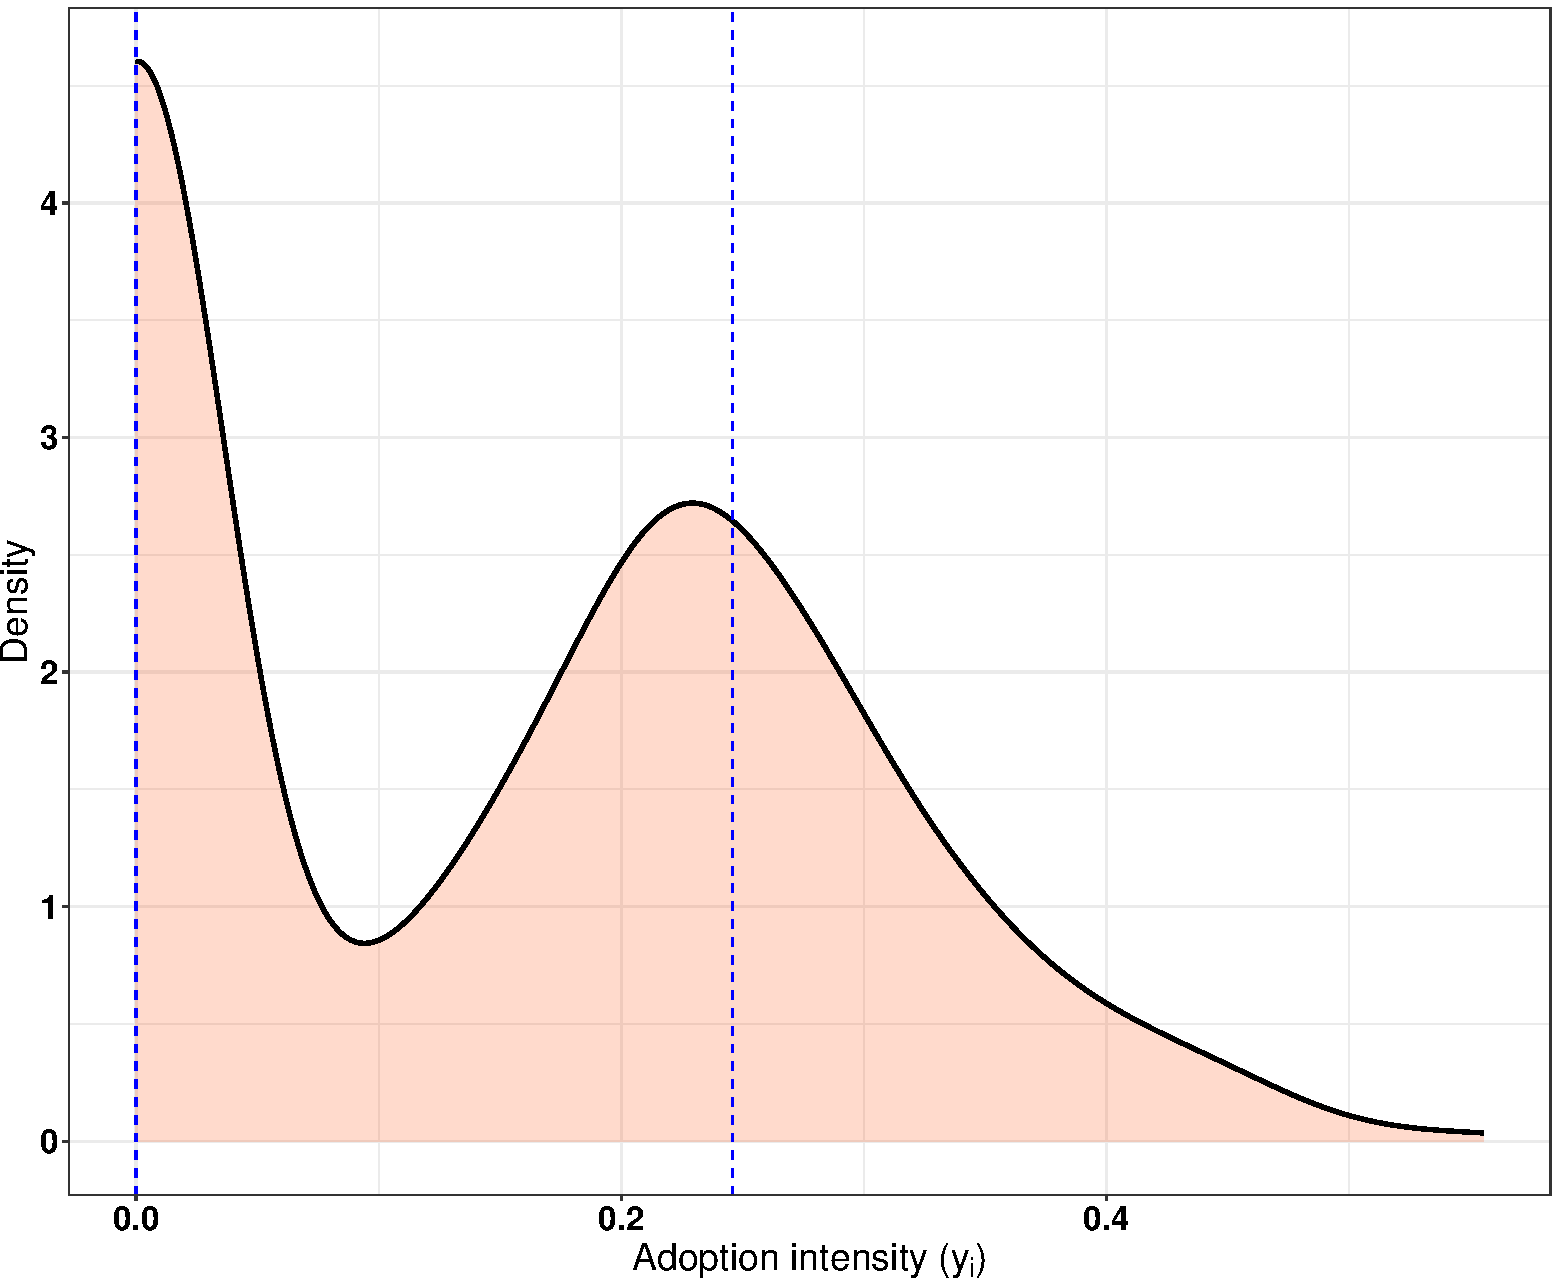
\includegraphics[width=0.8\textwidth]{density.pdf}
  \caption{Data-generating processes associated with sequential decision making}
  \label{fig:2}
  \smallskip
  \textbf{Source:} Survey Data (2023).
\end{figure} 

\subsubsection*{\textit{Part I of the decision process:  probability of adoption}}
The first part of the TP-FRM governs the adoption decision---a binary response determining whether an orchard manager adopts the APM. Conditional on awareness, adoption $a_i$ is defined as:
\begin{align}
(a_i | \mathbf{z}_i, w_i = 1) &= \begin{cases} 
1, & \text{if } a_i^* \in (0,1], \\
0, & \text{if } a_i^* = 0,
\end{cases}
\label{eq:5}
\end{align}
where $a_i^*$ is the latent adoption, $w_i$ is a binary variable indicating APM awareness (1 = aware), and $\mathbf{z}_i$ denotes a $1 \times K$ set of covariates hypothesised to influence the adoption decision. The probability of adoption is estimated using a probit and specified as:
\begin{align}
Pr(a_i = 1 | \mathbf{z}_i, w_i = 1) &= Pr(a_i^* \in (0,1]| \mathbf{z}_i, w_i = 1) = \Phi(\vartheta \mathbf{z}_i)
\label{eq:6}
\end{align}
where $\mathbb{E}(\cdot)$ is the expectations operator, $\Phi(\cdot) \equiv \int_{-\infty}^{z} \phi(v)dv$ is the standard normal cumulative distribution function (cdf), $\vartheta$ is a $K \times 1$ vector of parameters of interest.

Using the delta method, the average marginal effects (AMEs) for continuous and discrete covariates are estimated as (\cite{Papke2008}):
\begin{align}
\frac{\partial \mathbb{E}(a_i | \mathbf{z}, w_i = 1)}{\partial \mathbf{x}_j} = \vartheta_j \Phi(\vartheta \mathbf{z}) \equiv \vartheta_j \mathbb{E}[\Phi(\vartheta \mathbf{z})] \equiv \hat{\vartheta_j} \left[N^{-1} \sum_{i=1}^{N} \Phi(\hat{\vartheta} \mathbf{z}_i) \right]\\
\Phi(\vartheta z_{(1)}) - \Phi(\vartheta z_{(0)}) \equiv N^{-1} \sum_{i=1}^{N} \left[\Phi(\hat{\vartheta}z_{(1)}) - \Phi(\hat{\vartheta}z_{(0)}) \right]
\end{align}
\subsubsection*{\textit{Part II of the decision process: intensity of adoption}}
The second part of the TP-FRM pertains to the intensity decision. Conditional on awareness, the expected intensity of adoption $y_i$ is estimated by a fractional probit as:
\begin{align}
\mathbb{E}(y_i | \mathbf{x}_i, a_i^* &\in (0,1], w_i \in (0,1]) = G(\varphi \mathbf{x})
\label{eq:9}
\end{align}
where $\mathbf{x}_i$ is the $1 \times K$ set of regressors, $\varphi$ is the $K \times 1$ vector of parameters of interest, and $G(\cdot)$ is the Bernoulli specification of the quasi-maximum likelihood estimator (QMLE) specified as:
\begin{align}
l(\varphi;y_i;\mathbf{x}) = \arg \max_{\varphi} \sum_{i=1}^{N} [y_i \cdot \log(\Phi(\varphi \mathbf{x})) + (1 - y_i) \cdot \log(1 - \Phi(\varphi \mathbf{x}))]
\end{align}
The QMLE yields consistent $\varphi$s provided that Eqs.~(\ref{eq:6}) and (\ref{eq:9}) are not misspecified (\cite{Papke1996}). 

Given Eq.~(\ref{eq:9}), we are interested in the marginal effects of $x_i$ on the expected value of adoption intensity among adopters, weighted by the probability of adoption given that an orchard manager is aware of APM practices. These effects are henceforth referred to as conditional marginal effects (CMEs) and are estimated as:
\begin{align}
\begin{split}
& \mathbb{E}(y_i | \mathbf{x}_i, a_i^* \in (0,1], w_i = 1) \cdot Pr(a_i^* \in (0,1]|\mathbf{z}_i) = G(\varphi \mathbf{x}_i) \cdot \Phi(\vartheta \mathbf{z}_i) \\
& \frac{\partial \mathbb{E}(y_i|\mathbf{x}_i,a^*_i\in(0,1],w_i=1)}{\partial \mathbf{x}_j}{\Phi(\vartheta \mathbf{z})} + \frac{\partial Pr(a^*_i\in(0,1]|\mathbf{z}_i,w_i=1)}{\partial \mathbf{x}_j}{G(\varphi \mathbf{x})\varphi_j}
\end{split}
\end{align}

We also harvested the unconditional marginal effects (UCMEs) obtained as the marginal effect of $x_i$ for the total expected value of $y_i$ for the whole sample at the mean intensity: 
\begin{align}
\begin{split}
  \mathbb{E}(y_i | \mathbf{x}_i )\cdot Pr(a_i^* \in (0,1]|\mathbf{z}_i) = G(\varphi \mathbf{x}) \cdot \Phi(\vartheta \mathbf{z})\\
\frac{\partial \mathbb{E}(y|\mathbf{x})}{\partial \mathbf{x}_j}
= \frac{\partial G(\varphi \mathbf{x})}{\partial x_j} \Phi(\vartheta \mathbf{z}) + \frac{\partial \Phi(\vartheta \mathbf{z})}{\partial \mathbf{x}_j} G(\varphi \mathbf{x})
\end{split}
\end{align}

The TP-FRM model is attractive for several reasons. First, it allows for separate treatment of adoption and intensity decisions, which permits different covariates to have dissimilar effects at the adoption and intensity stages (\cite{Ramalho2009}). Second, the estimates obtained from the QMLE are always consistent since the conditional expectation is directly approximated based on the regressors (\cite{Papke1996}). Third, no special transformations are required to handle high probability masses at either extremum of the unit interval. Finally, the model accounts for nonlinearities and yields better fitted estimates when predicting response values within the [0, 1] limits of the response variable while controlling for non-constant effects of any regressor along its entire range (\cite{Papke1996}).

\subsection{Measurement of variables}
The study considered three types of intrinsic latent variables, including attitudes, perceptions and information constraints, as well as extrinsic covariates such as institutional and social factors, orchard-specific attributes, and resource endowment. Variable selection followed \textit{a priori} expectations based on the relevant empirical literature (\cite{Despotovic2019, Kabir2022, Midingoyi2019, Misango2022, Muriithi2021, Mwungu2020, Nyangau2022, Otieno2023, Sadique2022, Wangithi2021, Zeweld2017}). For brevity’s sake, a description of the individual variables is provided in Table~\ref{tab:1}. Latent attitudinal constructs were measured using several statements and were graded on five-point Likert scale items anchored from strongly disagree to strongly agree. The responses were then converted to scores with equal weighting. Farmers scoring half or more out of the total points were classified as having positive latent outcomes (attitudes or perceptions), while those scoring less than half were classified as having negative latent outcomes.

\section{Results and discussion}\label{sec:3} 
\subsection{Characteristics of the surveyed households}
Table~\ref{tab:1} presents the summary statistics of the surveyed households. To determine the mean differences between adopters and non-adopters, we utilised both two-sample \textit{t} tests and Pearson chi-square tests. The results indicate that the orchard management role was male-dominated at 71\%, conforming to the patriarchal nature of the community in the study area. A typical farmer belonged to the middle-aged category (54 years), and only 12\% of the orchard managers were youths (18--35 years). Eighty percent of the interviewed orchard managers were household heads, which supported our preference for the orchard manager as the unit of analysis. The average household consisted of 5 people, which aligns with the county average of 4 (\cite{County2022}).

The majority of the households (95\%) owned livestock, with an average tropical livestock unit (TLU) of 3. This is expected given the privatised, fragmented and limited land holdings in the study area. On average, an orchard manager allocated 1.34 acres of land to 61 mature trees, resulting in an average plant density of 45 trees per acre. Thus, most of the orchard managers were smallholders. Ninety percent of the cultivars grown were grafted hybrids, which are more preferred by the pest compared to traditional varieties. Knowledge deficits were notably prevalent among non-adopters, 83\% of whom faced this constraint.
\begin{sidewaystable}[htbp]
    \centering
    \caption{Characteristics of APM adopters and non-adopters}
    \label{tab:1}
    \small
    \begin{adjustbox}{width=1\textwidth, center}
        \begin{tabular}{l >{\raggedright\arraybackslash}p{8cm} ccccc}
            \toprule
            & & Pooled & Adopters (a) & Non-adopters (b) & \multicolumn{2}{c}{Test of statistical differences (a-b)}\\
            \cmidrule(lr){3-3} \cmidrule(lr){4-5} \cmidrule(lr){6-7}
            Variable & Description & Mean (SD) & Mean (SD) & Mean (SD) & Diff. & \textit{t}-test\\
            \midrule
            \textbf{\textit{Continuous variables}} & & & & & & \\
            Age & Age of the orchard manager (years) & 53.586 (14.620) & 53.707 (14.649) & 53.421 (14.619) & 0.286 & 0.201 \\
            Household size & Number of household members (count) & 5.134 (2.562) & 5.265 (2.733) & 4.956 (2.303) & 0.309 & 1.239 \\
            Neighbours & Number of adopting neighbours (count) & 8.162 (11.291) & 10.129 (13.135) & 5.486 (7.372) & 4.620 & 4.308*** \\
            Orchard size & Land under mango production (acres) & 1.342 (1.105) & 1.445 (1.158) & 1.202 (1.015) & 0.243 & 2.267** \\
            Producing trees & Number of mango trees in production (count) & 60.863 (73.180) & 72.863 (85.971) & 44.536 (46.324) & 28.328 & 4.046*** \\
            TLU & Tropical livestock units (index) & 3.068 (3.188) & 3.369 (3.608) & 2.659 (2.458) & 0.710 & 2.298** \\
            Quality of awareness & Proportion of APM practices the orchard manager is aware of to the total practices (proportion) & 0.385 (0.175) & 0.403 (0.174) & 0.361 (0.174) & 0.042 & 2.494** \\
            \midrule
            \textbf{\textit{Categorical variables}} & & Proportions & & & & $\chi^2$ test\\
            \midrule
            Gender & Orchard manager is a male (\%) & 70.6 & 73.5 & 66.7 & 6.8 & 2.369 \\
            Biodiversity & Positive attitude towards orchard biodiversity (\%) & 93.3 & 95.2 & 90.7 & 4.5 &3.366*\\
            Severity & Fruit fly severity is rated as severe (\%) & 56.9 & 55.8 & 58.5 & -2.6 & 0.301 \\
            Prospects & Positive attitude towards orchard prospects (\%) & 92.8 & 92.8 & 92.9 & -0.1 & 0.003\\
            Perceived benefit & Positive perception on the benefits of APM to suppress fruit fly (\%) & 82.6 & 89.2 & 73.8 & 15.4 & 17.405***\\
            Perceived ease of use & Positive perception on the ease of use of APM (\%) & 87.7 & 90.4 & 84.2 & 6.2 & 3.777*\\
            Pesticide effectiveness & Positive perception of the ability of synthetic pesticides to control fruit fly (\%) & 97.0 & 98.4 & 95.1 & 3.3 & 3.963**\\
            Off-farm income & Accessed income from non-agricultural streams (\%) & 76.9 & 75.1 & 79.2 & -4.1 & 1.014\\
            Co-creation & Participated in co-creation activities (\%) & 44.7 & 48.6 & 39.3 & 9.3 & 3.651*\\
            Group membership & A member of a farmer group (\%) & 38.0 & 45.8 & 27.3 & 18.5 & 15.264***\\
            Training on pest management & Accessed training on pest management (\%) & 25.9 & 32.1 & 17.5 & 14.6 & 11.775***\\
            Knowledge constraint & Limited expertise on the implementation of APM (\%) & 39.8 & 8.4 & 82.5 & -74.1 & 335.637***\\
            \midrule
            $N$ & & 432 & 249 & 183 & & \\
            \bottomrule
        \end{tabular}
    \end{adjustbox}
    \smallskip
    \parbox{.9\textwidth}{\textit{Note:} *, **, and *** denote statistical significance at the 10, 5, and 1\% levels, respectively. The values in parentheses are standard deviations. The TLU conversion factors utilised were as follows: cattle (0.70), calf (0.25), donkey (0.50), sheep (0.10), goat (0.08), pig (0.20), rabbit (0.01), and poultry (0.01) (\cite{FAO1993}).\\
        \textbf{Source:} Survey Data (2023).}
\end{sidewaystable}

\subsection{Adoption and intensity of the APM}
Table~\ref{tab:2} provides an overview of the uptake of the 18 APM practices considered in this study. Almost all respondents (98\%) utilised synthetic insecticides to control fruit fly. However, only 56.7\% of the farmers adopted APM. On average, a farmer was aware of 2 out of the 6 reactive APM practices, which could be the reason behind the limited uptake of the technology. Only 3 (16.7\%) of the practices were adopted by more than half of the respondents. Most of the respondents (85\%) confirmed access to protective gear, 83\% of whom utilised them when applying pesticides. About 68\% of the orchard managers reported always reading pesticide labels before use, while 41\% were unaware of adulterated, banned, counterfeit or unregistered products.

\begin{table}[!ht]
\begin{threeparttable}[b]
  \centering
  \caption{Adoption of APM technology components for fruit fly management ($n=432$)}
  \label{tab:2}
  \begin{tabularx}{\textwidth}{@{}lXlXc@{}}
    \toprule
    \textbf{Category} & \textbf{Component} & \textbf{APM Practice} & \textbf{\% of adopters}\\
    \midrule
    \multirow{6}{*}{\textit{Reactive options}}& \multirow{6}{=}{Biological control and bio-derived products}& Male annihilation & 50.2 \\
    & & Smoking herbs and dung & 14.4 \\
    & & Spraying botanical pesticides (concoctions) & 4.2 \\
    & & Spot spray of food baits & 1.6 \\
    & & Soil inoculation with biopesticides & 0.5 \\
    & & Spraying ash/baking powder and tobacco & 0.5 \\
    & & Release of ovivorous ants and parasitoid wasps\tnote{*} & - \\
    \midrule
    \multirow{12}{*}{\textit{Preventive options}}& \multirow{6}{=}{Orchard sanitation}& Feeding infested fruits to livestock & 45.6 \\
    & & Deep burying infested fruits & 35.2 \\
    & & Composting infested fruits & 17.1 \\
    & & Burning infested fruits & 6.9 \\
    & & Solarisation with special ``solar'' bags & 3.2 \\
    & & Use of an augmentorium & 0.2 \\
    \cmidrule(lr){2-4}
    & \multirow{7}{=}{Habitat management}& Regular scouting and monitoring & 53.5 \\
    & & Proper management of alternate hosts & 50.2 \\
    & & Inter-tree raking & 43.3 \\
    & & Intercropping with non-host crops & 13.4 \\
    & & Early harvesting & 13.0 \\
    & & Trap cropping with passion fruits & 2.1 \\
    \bottomrule
  \end{tabularx}
  \begin{tablenotes}
      \item [*] \small Biological pest control through natural enemies is often associated with ecological processes on larger scales than at the orchard-level. Additionally, this practice is self-spreading and is implemented at no cost to the farmer (\cite{Korir2015}). Therefore, we did not consider it in the current study.
  \end{tablenotes}
  \smallskip 
  \textbf{Source:} Survey Data (2023).
  \end{threeparttable}
\end{table}

The APM options are synergistic and complementary---the adoption of additional practices synergises pest suppression efforts. We observed low intensities of adoption (Figure~\ref{fig:3}), with only 0.5\% of the orchard managers using more than half of the practices concurrently. While the most intensive adopter incorporated approximately 56\% of the practices, the average adopter utilised only 25\% of the options.
\begin{figure}[!ht]
  \centering
  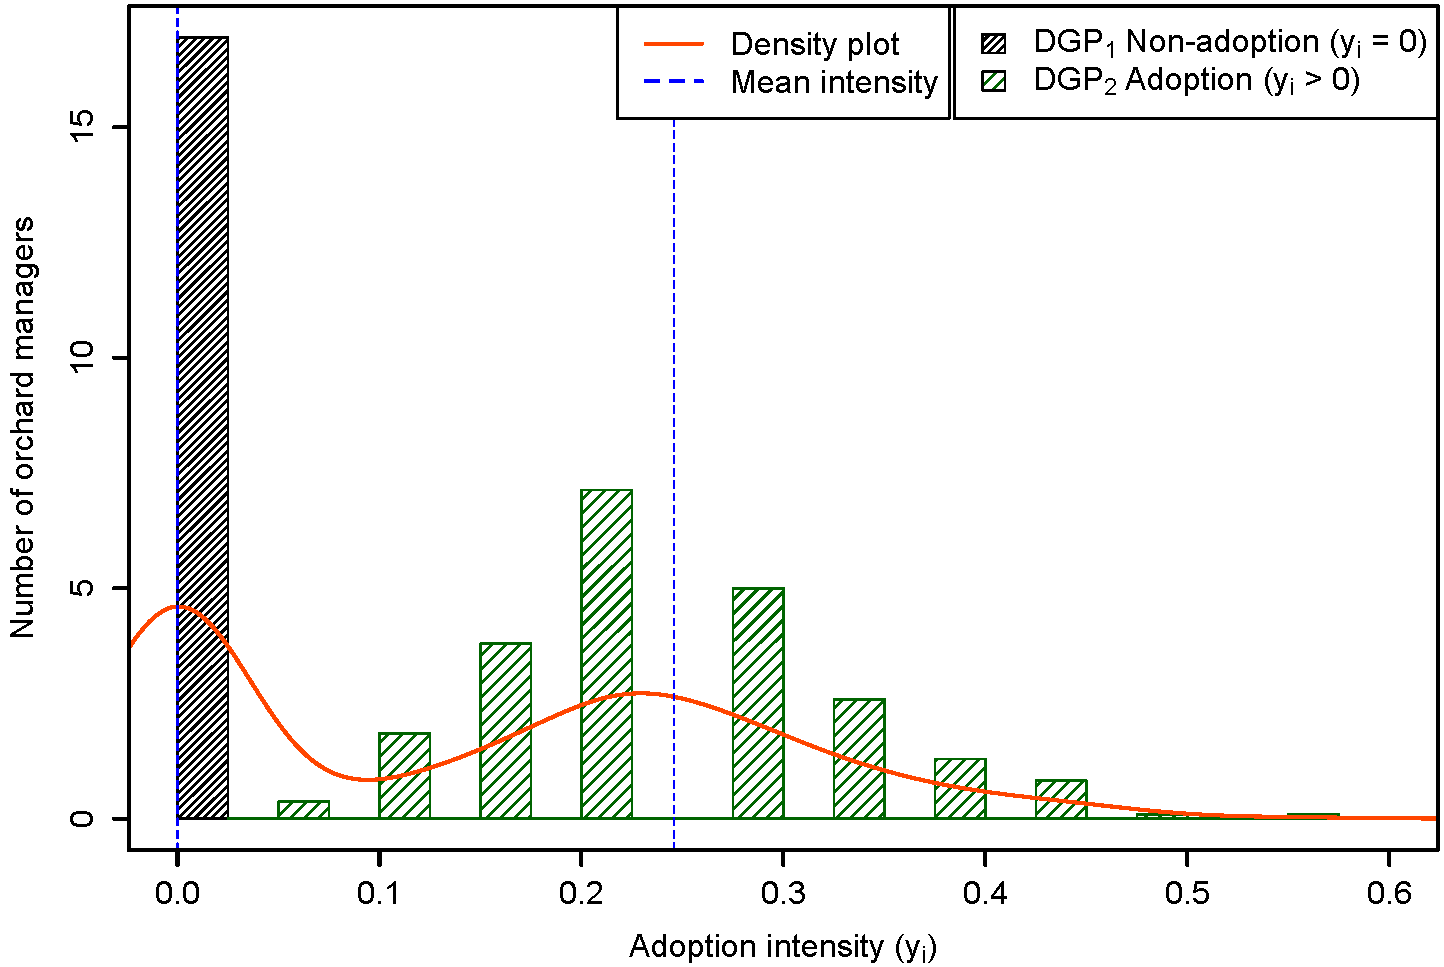
\includegraphics[width=1\textwidth]{intensity_2.pdf}
  \caption{Intensity of adoption of agroecological pest management options}
  \label{fig:3}
  \smallskip
  \textbf{Source:} Survey Data (2023).
\end{figure} 

\subsection{Empirical results}
\subsubsection{\textit{Model selection}}
Table~\ref{tab:3} outlines the model diagnostics for the TP-FRM. The robust goodness-of-functional-form (GGOFF) test proposed by \cite{Ramalho2011} and \cite{Ramalho2014} failed to reject our probit link specification. Similarly, the robust \cite{Ramsey1969} regression-equation specification-error test (RESET) confirmed the absence of omitted variable bias. Since our censoring mechanism yields genuine zeros for non-adopters, no exclusion restrictions were necessary for model identification. No multicollinearity was observed in the data, as indicated by the mean variance inflation factor (VIF) test coefficient of 1.18 (against the critical value of 10). Regression models on semi-continuous variables with finite boundary observations always exhibit non-constant error variance (\cite{Papke1996}). Therefore, we did not need to test for heteroskedasticity, and the QMLE inherently handles this problem. Overall, the covariates employed in this study explained 37.2\% of the variation in both adoption and intensity decisions. All analyses were performed in R and Stata version 18.
\begin{table}[htbp]
\centering
\caption{Model diagnostics for the TP-FRM}
\label{tab:3}
\begin{tabularx}{0.8\textwidth\center}{lXcc}
\hline
& & \textbf{Part I:} \textit{Probit} & \textbf{Part II:} \textit{Fractional probit} \\
\cmidrule(lr){3-3} \cmidrule(lr){4-4}
Test & Version & Statistic (\textit{p}-value) & Statistic (\textit{p}-value)\\
\hline
Robust RESET & LM & 1.513 (0.219) & 0.004 (0.947) \\
Goodness of functional form & LM & 3.999 (0.135) & 3.488 (0.175) \\
 & Wald & 2.831 (0.243) & 3.321 (0.190) \\
 & LR & 2.788 (0.248) & - \\
Overall R$^2$ type measure & & 0.372 & \\
Mean VIF & & 1.21 & \\
\hline
$N$ & & 423 & 249 \\
\hline
\end{tabularx}
\smallskip
    \parbox{0.7\textwidth}{\small\textit{Note:} Values in parentheses are \textit{p}-values. Abbreviations: LM, Lagrangian multiplier; RESET, regression-equation specification-error test; LR, likelihood ratio; VIF, variance inflation factor.}\\
    \textbf{Source:} Survey Data (2023).
\end{table}

\subsubsection{\textit{Determinants of adoption of APM practices}}
The results of the first part of the TP-FRM governing the adoption decision are presented in Table~\ref{tab:4} columns 2 and 3. Our probit results suggested that, conditional on APM awareness, APM adoption was positively influenced by perceived benefit of APM, number of producing trees, group membership, and access to training on pest management. Only orchard size had a significant negative effect on the probability of adoption.
\begin{table}[!ht]
\centering
\caption{Estimates of the TP-FRM for adoption and intensity decisions}
\label{tab:4}
\begin{adjustbox}{width=1\textwidth, center}
\begin{tabular}{lcccccc}
\toprule
& \multicolumn{2}{c}{\textbf{Part I: Adoption}} & \multicolumn{4}{c}{\textbf{Part II: Intensity of adoption}} \\
& \multicolumn{2}{c}{(\textit{Probit})} & \multicolumn{4}{c}{(\textit{Fractional probit)}} \\
\cmidrule(lr){2-3} \cmidrule(lr){4-7}
& & Robust & & Robust & & Robust \\
Variable & AME & Std. Err. & CME & Std. Err. & UCME & Std. Err. \\
\midrule
\textbf{Demographic factors} \\
Age & 0.000 & 0.002 & -0.001** & 0.000 & -0.001** & 0.000 \\
Gender & 0.091* & 0.048 & 0.031*** & 0.011 & 0.029*** & 0.010 \\

\textbf{Resource endowment} \\
Household size & 0.007 & 0.009 & -0.001 & 0.002 & -0.001 & 0.001 \\
Off-farm income & -0.003 & 0.054 & 0.007 & 0.011 & 0.006 & 0.010 \\
TLU & 0.007 & 0.008 & 0.002* & 0.001 & 0.002* & 0.001 \\

\textbf{Attitudes} \\
Biodiversity & 0.139 & 0.099 & 0.066*** & 0.024 & 0.062*** & 0.022 \\
Severity & -0.071 & 0.046 & -0.015 & 0.010 & -0.014 & 0.009 \\
Prospects & -0.008 & 0.088 & 0.063*** & 0.018 & 0.059*** & 0.016 \\

\textbf{Perceptions} \\
Perceived benefit & 0.191*** & 0.060 & -0.015 & 0.016 & -0.014 & 0.015 \\
Perceived ease of use & 0.126* & 0.068 & -0.031* & 0.017 & -0.029* & 0.016 \\
Pesticide effectiveness & 0.222* & 0.129 & -0.045*** & 0.017 & -0.042*** & 0.016 \\

\textbf{Orchard-specific factors} \\
Orchard size & -0.052** & 0.026 & -0.002 & 0.004 & -0.002 & 0.004 \\
Producing trees & 0.002*** & 0.000 & 0.000 & 0.000 & 0.000 & 0.000 \\

\textbf{Institutional and social factors} \\
Neighbours & 0.006* & 0.004 & 0.002*** & 0.000 & 0.002*** & 0.000 \\
Co-creation & 0.067 & 0.045 & 0.035*** & 0.010 & 0.033*** & 0.009 \\
Group membership & 0.116** & 0.048 & 0.021* & 0.011 & 0.020* & 0.010 \\
Training on pest management & 0.119** & 0.053 & 0.011 & 0.011 & 0.010 & 0.011 \\

\textbf{Information constraints} \\
Quality of awareness & & & 0.074*** & 0.027 & 0.069*** & 0.025 \\
Knowledge constraint & & & -0.049*** & 0.017 & -0.046*** & 0.015 \\
Constant & -2.382*** & 0.663 & -0.995*** & 0.137 &\\ 
\midrule
\textbf{\textit{Goodness of fit statistics}} \\
Log pseudo-likelihood & -245.946 & & -94.164 & & & \\
Deviance & 491.892 & & 7.147 & & & \\
Pearson & 421.059 & & 7.036 & & & \\
$R^2$ type measure & 0.175 & & 0.307 & & & \\
AIC & 1.248 & & 0.917 & & & \\
BIC & -1957.293 & & -1256.349 & & & \\
\midrule
N & 423 & & 249 & & & \\
\bottomrule
\end{tabular}
\end{adjustbox}
\smallskip
    \parbox{0.9\textwidth}{\small\textit{Note:} : *, **, and *** denote statistical significance at the 10, 5, and 1\% levels, respectively. Abbreviations: AME, average marginal effect; AIC, Akaike information criterion; BIC, Bayesian information criterion; CME, conditional marginal effect; UCME, unconditional marginal effect.\\
    \textbf{Source:} Survey Data (2023).}
\end{table}

It is well established that producers adopt technologies more readily when they are associated with economic gains. Our results support these expectations and suggest that farmers who perceived the APM technology as beneficial for suppressing fruit flies, reducing management costs, and reducing health risks were 19.1\% more likely to adopt it. This finding conforms to the results of \cite{Kabir2022}, who found a positive association between perceived benefit and adoption of integrated pest management (IPM), a subset of APM. \cite{Zeweld2017} also reported a positive relationship between perceived usefulness and farmers’ intention to adopt sustainable practices.

Interestingly, having a positive perception of the effectiveness of synthetic pesticides in fruit fly suppression was associated with an increase in the probability of APM adoption (significant at the 10\%). Since APM involves the synergistic integration of control strategies, the framework may improve the effectiveness of synthetic pesticides when used within the ‘mix,’ leading to the observed positive influence. Consistent with this finding, \cite{Muriithi2021} reported that the perceived effectiveness of pesticides increased the odds of willingness to pay for the IPM strategy among farmers in Ethiopia. 

The relationship between information-seeking behaviour and adoption is well known to be positive. Our findings agreed with these expectations and suggested an 11.9\% increase in the likelihood of adoption among trained farmers. Extant studies on fruit fly IPM, such as those of \cite{Midingoyi2019}, \cite{Mwungu2020}, \cite{Wangithi2021}, and \cite{Otieno2023}, have revealed similar effects. Training influences adoption indirectly through the creation of awareness, the formation of attitudes and perceptions, and the reduction of knowledge deficits, leading to a positive effect.

Affiliation with a group increased the likelihood of APM adoption by 11.6\%. Membership in groups improves access to inputs and product markets and facilitates information transfer through social learning. Although similar conclusions have been reached by some studies (for example, \cite{Kabir2022, Midingoyi2019, Otieno2023}), \cite{Mwungu2020} reported a negative association between fruit fly IPM adoption and membership in agricultural groups. This unexpected finding could be associated with the reverse effects of social groups such as free-riding, which are not uncommon in large group settings.

Our findings suggested that farmers with many mango trees were more likely to be adopters than were those with fewer trees. These findings align with the results of \cite{Korir2015} and \cite{Mwungu2020}, who reported a significant and positive influence of the number of mature trees on IPM adoption. Producers with a large number of trees are more likely to be commercialised, prioritising cost-effective practices that alleviate overdependence on often-expensive synthetic pesticides.

The relationship between land size and the adoption of sustainable pest management technologies is inconclusive in the literature. Our results suggested an inverse association between APM adoption and orchard size. \cite{Despotovic2019} also found that farm size negatively influenced the intention to adopt IPM. As a divergence, \cite{Mwungu2020} and \cite{Wangithi2021} reported a positive relationship between mango orchard area and the adoption of fruit fly IPM in Kenya. \cite{Sadique2022} also reported a positive association between land size and IPM adoption by vegetable farmers in Bangladesh. Farmers with larger farms are usually more oriented towards commercialised production and may be less likely to adopt alternative technologies due to the risks of yield loss.

\subsubsection{\textit{Drivers of the intensity of APM adoption}}
Columns 4 to 7 of Table~\ref{tab:4} summarise the results from the second part of the TP-FRM for drivers of intensity of adoption. Both the CMEs and UCMEs were consistent across all covariates, except that the former predicted relatively small effects with slightly more precise standard errors. However, since we were interested in the effects of the covariates after controlling for awareness, we focus the ensuing discussion on the CMEs. The results suggested that gender, attitude towards orchard biodiversity, attitude towards orchard prospects, number of adopting neighbours, knowledge co-creation with fellow farmers, and quality of awareness had significant positive effects on the intensity of adoption. On the other hand, age, perceived pesticide effectiveness and knowledge constraints significantly reduced the intensity of adoption.

As hypothesised, the quality of awareness had a significant positive effect on the intensity of adoption. For every percentage increase in the quality of awareness, the extent of adoption increased by 7.4\% \textit{ceteris paribus}. Increased exposure to APM practices offers orchard managers the flexibility to choose from a wider range of complementary practices. Thus, farmers are likely to adopt more practices as they become exposed to more technology components. Similarly, \cite{Tambo2023} reported that recipients of information were more inclined to adopt multiple nonchemical fall armyworm control strategies. We also observed that orchard managers with limited expertise in APM implementation were likely to adopt the technology 4.9\% less intensively than were those without this constraint. This aligns with expectations since APM technology is knowledge intensive. \cite{Despotovic2019} and \cite{Wangithi2021} also arrived at similar conclusions. Poor expertise increases the uncertainty associated with intensive adoption of APM, reinforcing confidence in conventional methods.

In conformity with \textit{a priori} expectations, a positive attitude toward orchard biodiversity was associated with 6.6\% higher adoption intensity among orchard managers. Farmers who value orchard biodiversity as a method of pest control are more likely to adopt biodiversity-enhancing practices, such as agroforestry and the cultivation of companion crops, which favour the existence of natural enemies, reinforcing overall pest management efforts. Our findings also revealed that a positive attitude toward orchard prospects resulted in a 6.3\% increase in the intensity of adoption, suggesting that orchard managers who intended to quit mango production were likely to adopt fewer APM components. Uncertainties regarding farm prospects may lead to reduced adoption levels, particularly when the technology has more relative advantages in the long run, as is the case for APM technology.

Although the probit model suggested that having a positive perception of the ease of use of APM technology increased the likelihood of its adoption, interestingly, the effect was negative for intensity of adoption (at the 10\%). This suggest that orchard managers who perceive the technology as less complex to implement were likely to adopt the technology albeit, post-adoption, those who still had the same perception were likely to be those who adopted the technology less intensively. The complexity of the implementation of APM technology increases with more intensive adoption and application at wider scales. Therefore, more intensive adopters are likely to perceive the technology as more difficult to implement and maintain given its high labour and skills requirements compared to less intensive users. \cite{Zeweld2017} also observed a negative association between perceived ease of adoption and intention to adopt sustainable practices such as minimum tillage.

A positive perception of the effectiveness of inorganic pesticides for suppressing fruit flies was associated with a 4.5\% decrease in the intensity of APM adoption. These findings corroborate the findings of \cite{Schreinemachers2017}, who reported that farmers who believed in the effectiveness and indispensability of synthetic pesticides increased their use despite being aware of their health impacts. Orchard managers who perceive synthetic pesticides as effective at suppressing fruit flies are likely to adopt APM technology less intensively due to greater reliance on synthetic pesticides, diminishing the finite resources that can be allocated to APM. 

Participation in co-creation activities with fellow farmers increased the extent of APM adoption by 3.5\%. Information-sharing activities among farmers enhance the awareness and expertise necessary for intensive adoption of the APM strategy. A similar pattern was observed by \cite{Schreinemachers2017}, who noted that pesticide usage decreased when farmers consulted fellow friends or neighbours. In contrast, \cite{Murage2015} found that the rates of IPM adoption decreased when farmers received first information on the technology from an early adopter. However, their finding was relative to when farmers received information from extension officers, who are expected to have more information than early adopters.

Being a male orchard manager was associated with a 3.1\% increase in APM adoption intensity, suggesting that females adopted the technology less intensively than males did. This could be attributed to potential challenges faced by female orchard managers, such as heavier household workloads and limited access to essential services such as extension and credit, which may lead to time, information, and liquidity constraints. Additionally, in most patriarchal SSA communities, male privilege offers greater access to and control over joint household resources such as livestock that facilitate household and farm financial decisions. In line with these findings, \cite{Muriithi2021} reported that males were more willing to pay for fruit fly IPM. This finding is also consistent with the results of \cite{Wangithi2021} and \cite{Otieno2023}, who also reported that male farmers were more likely to be continued users of the fruit fly IPM. This finding agrees with the results of \cite{Murage2015}, who established a positive correlation between gender and the intensity of adoption of climate-smart push-pull technology in Kenya. This result is also in accordance with the findings of \cite{Misango2022}, who revealed that males committed more land to push-pull technology in Rwanda.

The extent of APM adoption increased with increased number of adopting neighbours. Neighbourhood effects can alleviate common barriers to intensive adoption of eco-friendly practices, such as poor awareness and expertise and inadequate resources, by harnessing social capital. Moreover, social dynamics such as peer effects and reputation can also improve the rate of uptake of innovations such as APM. Neighbouring farms exert peer pressure among farmers due to the perceived need for social comparison within the locality. It has been observed that if the participation of nearby farmers reaches a substantial threshold, non-adopters might perceive this cue as the descriptive norm or may want to adopt it for social comparison purposes (\cite{Despotovic2019, Dessart2019, Ejelov2022}). Intensive adoption by reputable neighbouring farms may also serve as a cue that encourages others to adopt it more intensively. Similar findings were reported by \cite{Misango2022} and \cite{Alhassan2023}. Results of our probit model also revealed that the number of adopting neighbours increased the probability of APM adoption (although significant at the 10\%), corroborating the results of \cite{Midingoyi2019}, who found that knowledge of more neighbours who were adopters within the farmer’s vicinity increased the probability of uptake of fruit fly IPM. \cite{Bakker2021} also reported that descriptive norms associated with neighbourhood connections positively influence farmers’ intentions to reduce pesticide usage and opt for sustainable alternatives.  

Older farmers were inclined to adopt fewer APM practices than were their younger counterparts. This finding aligns with those of \cite{Kabir2015} that older farmers in Bangladesh adopted IPM vegetable farming less intensively than younger farmers did. \cite{Nyangau2022} also reported a lower willingness to pay for bio-pesticides among older farmers in Uganda, while \cite{Kabir2022} observed that older producers had a lower willingness to adopt botanical pesticides. The labor-intensive nature of APM makes younger, more energetic farmers more likely to adopt it intensively. Moreover, older farmers may be attached to traditional practices and may be reluctant to deviate from what has worked in the past. 

\section{Conclusions and policy implications}\label{sec:4}
Mango production and marketing in Kenya are impeded by \textit{B. dorsalis} invasion, which has led farmers to heavily depend on synthetic pesticides. Since the trade-offs between pesticide usage and socio-environmental risks are inextricable, eco-friendly control methods such as APM have been encouraged. This study assessed the drivers of the transition towards the APM for mango fruit fly suppression among smallholders. The results suggest a high dependence on synthetic pesticides (98\%) and low APM adoption rates (56.7\%), with the average adopter utilising only 25\% of the practices concurrently. This low uptake can be attributed to the high knowledge deficit in the implementation of APM technology, particularly among non-adopters (83\%). The findings from the two-part fractional regression model indicate that both the decisions to adopt and the extent of adoption of APM were primarily motivated by socio-psychological attributes of the decision maker. While the perceptions of technology attributes and information-seeking behaviour primarily influenced the adoption decision, attitudes toward orchard biodiversity and prospects, as well as information constraints, were the main drivers of the intensity of adoption. 

We recommend that policymakers consider incentives that appeal to farmers’ intrinsic motivations when designing agro-ecological policies and interventions. Opportunities for farmer training and co-creation of knowledge should increase, with a specific focus on gender-disaggregated participatory group approaches such as farmer field schools and co-design workshops. Both training and co-creation activities should aim to increase awareness of the relative advantages of APM technology by providing a noncomplex understanding of its principles and implementation through ‘observation- and discovery-based’ learning. Interventions should capitalise on building local social networks, promoting interpersonal knowledge transfer, strengthening social capital, and harnessing farmers’ innovative capacities. Synergistic effects between various practices should be emphasised at the outset of such interventions. Older orchard managers and women should be considered the primary beneficiaries of these activities.

This study is not without limitations. We utilised cross-sectional data, which precluded the use of dynamic selection-on-observable estimators. However, future research could account for the dynamic effects of time-variant behavioural attributes along the transition pathway. We also refrained from including awareness as the initial stage of the sequential decision process due to data limitations. Future studies with larger samples and diverse variables could include this stage to derive more insights.

\subsection*{Acknowledgement}
The authors thank all respondents who participated in this study as well as the enumerators who generously collected the data.

\subsection*{Disclosure statement}
The authors declare no conflicts of interest.

\subsection*{ORCiD}
Sulman Olieko Owili \textcolor{blue}{\href{https://orcid.org/0000-0001-7401-5326}{https://orcid.org/0000-0001-7401-5326}}\\
David Jakinda Otieno \textcolor{blue}{\href{https://orcid.org/0000-0001-9904-0819}{https://orcid.org/0000-0001-9904-0819}}

\subsection*{Data availability statement}
The data utilised in this study are available from the corresponding author upon request.

\subsection*{Funding details}
This work was funded by the CGIAR Initiative on Agroecology.
\printbibliography
\end{document}
